\section{Moravec}\label{sec:moravec}
%Moravecs hjørnedetektor\cite{moravec}, er en af de tidligste feature detektorer og i denne metode defineres et hjørne, som et dataindsamlingsvindue i et billede $I$, der er forskelligt fra dets lokalområde. <?>
Moravecs hjørnedetektor\cite{moravec}, er en af de tidligste feature detektorer. Moravec definere et hjørne ved at placere et kvadratisk dataindsamlingsvindue over et punkt, hvorefter dette vindue forskydes med én pixel i alle principielle retninger (horisontalt, vertikalt, diagonalt). Forskellen imellem det originale og de forskudte vinduer observeres, og en stor forskel imellem vinduerne indikere et hjørne. Forskellen imellem de forskudte vinduer findes ved at estimere auto-korrelationen imellem det originale og de forskudte vindue. Denne auto-korrelation, eller intensitetvariation, estimeres ved SSD (Summed Square Difference):
\begin{equation}
\bold{E}_{u,v}(x,y)= \sum_{\forall \text{x,y i dataindsamlingsvinduet}} w(x,y)[I(x+u,y+v) - I(x,y)]^2
\label{moravec}     
\end{equation}
hvor $(u,v)\in \lbrace -1,0,1 \rbrace$ er sættet af forskydninger af vinduet.
%<$w$ er her en matrix<?>, med samme størrelse som $I$ <??> og indeholder 1 indenfor hvis en pixelkoordinat $(x,y)$ ligger indenfor dataindsamlingsvinduet, og 0 ellers<?>.>
Figur \ref{fig:moravec} illustrere et dataindsamlingsvindue af størrelse $3\times3$ (markeret med rød). Det blå vindue viser et diagonalt skift af dataindsamlingsvinduet med $(u,v)=(1,1)$.
\begin{figure}[H]
    \centering
    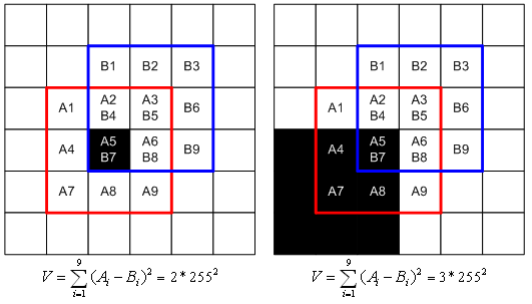
\includegraphics[width=0.55\textwidth]{fig/25.png}
     \vspace{-1em}
    \begin{center}    
       \caption{{\footnotesize \textit{SSD udregninger for to forskellige scener. (venstre) et dataindsamlingsvindue placeret på en mørk pixel. (højre) et dataindsamlingsvindue placeret et hjørne. }}}
    \label{fig:moravec}
     \end{center}
     \vspace{-2.5em}
  \end{figure} \noindent   
Hvert skift af $(u,v)$ fra ligning \eqref{moravec} returnere en intensitetsvariation. Den mindste af de otte variationer, definere punktets hjørnestyrke $C(x,y)$.
\begin{equation}
C(x,y)=min(\bold{E}_{u,v}(x,y)),\text{ }\forall S_{(u,v)} \in \lbrace-1,0,1\rbrace \backslash \lbrace0,0\rbrace
\end{equation}
En horisontal kant vil resultere i en lav intensitetsvariation med et dataindsamlingsvindue forskudt horisontalt derfor, for at identificere hjørner, tages minimum af $\bold{E}$ for at sikre en stor auto-korrelation i alle retninger.
%<vil have et højt respons i de områder, hvor pixelintensiteter i originalvinduet ($w(x,y) = 1$) <?>, adskiller sig fra intensiteter, i de forskudte vinduer - jo større pixelintensitens forskellen er, jo højere $C$ værdi.
Det kan udledes her, at en kant placeret langs en de principielle retninger, ikke vil blive karakteriseret som et hjørne da disse vil have  en lav auto-korrelation. Der opstilles en grænseværdi $t$ for $C$, der bestemmer om punktet er et hjørne(sandt/falsk) og derved om det kan udvælges som et interessepunkt.
\begin{equation}
\begin{split}
\text{hjørne} = 
\begin{cases}
\text{sandt}& \text{hvis } C(x,y)\geq t, \\
\text{falsk }& \text{hvis } C(x,y) < t.
\end{cases}
\end{split}
\label{cornerind}
\end{equation}
\subsubsection*{Algoritme: Moravec Detektor}
\begin{tabbing}
Input\quad \= : \= Billede $I$\\
Output \text{ } \> : \> Interessepunkter $p \in (x,y)$.
\end{tabbing}
\begin{enumerate}
\item{For hvert pixel i billedet, udregnes auto-korrelationen imellem hvert skift af $(u,v) \in \lbrace-1,0,1\rbrace$, udregnet ved ligning \ref{moravec}.}
\item{Hjørnestyrken udledes, ved at tage $C(x,y)=min(\bold{E}_{u,v}(x,y))$}
\item{Punkter der ikke overholder en opstillet grænseværdi for $C(x,y)$ fjernes.}
\end{enumerate}
\subsection*{Konklusion}
Moravec er en simpel algoritme, med mange udfordringer, og anvendes derfor ikke udbredt i praksis. Dette skyldes Moravecs antagelser om billedets natur:
\begin{itemize}
\item{Kanter forekommer i de principielle retninger.}
\item{Der er ingen støj i billedet.}
\end{itemize} 
Naturligt kan kanter forekomme i alle retninger og ikke kun i de principielle, som algoritmen tager højde for. Derudover er metoden følsom overfor støj i billedet. Forskydes vinduet, illustreret i figur \ref{fig:moravec} (venstre), vil intensitetsvariation være ens for alle forskydninger. Deformationer i billedet, som støj, kan derved fejlagtigt detekteres som hjørner.